\documentclass[
  12pt,
  openright,
  oneside,
  a4paper,
  english,
  brazil
]{abntex2}

\usepackage[T1]{fontenc}
\usepackage[utf8]{inputenc}
\usepackage{lmodern}
\usepackage{microtype}
\usepackage{indentfirst}
\usepackage{graphicx}
\usepackage{tikz}
\usetikzlibrary{arrows.meta,positioning}
\usepackage{booktabs}
\usepackage{longtable}
\usepackage{array}
\usepackage{tabularx}
\usepackage{enumitem}
\usepackage{url}
\usepackage{xurl}
\usepackage[alf]{abntex2cite}
\usepackage{hyperref}

\hypersetup{
  pdftitle={Inteligência Artificial de Baixo Consumo para o Monitoramento Preventivo do Bem-Estar Estudantil},
  pdfauthor={Ivo Calado; Rafael Durelli; Diego Dias},
  colorlinks=true,
  linkcolor=black,
  citecolor=black,
  urlcolor=blue,
  bookmarksdepth=4
}

\setlength{\parindent}{1.25cm}
\setlength{\parskip}{0.2cm}
\OnehalfSpacing
\setlist[itemize]{noitemsep,topsep=4pt}
\setlist[enumerate]{noitemsep,topsep=4pt}
\AtBeginEnvironment{longtable}{\small}
\Urlmuskip=0mu plus 1mu

\newcolumntype{Y}{>{\raggedright\arraybackslash}X}

\titulo{Inteligência Artificial de Baixo Consumo para o Monitoramento Preventivo do Bem-Estar Estudantil em Escolas Públicas de Baixa Conectividade}
\autor{Ivo Calado \\ Rafael Durelli \\ Diego Dias}
\local{Alagoas}
\data{2026}
\instituicao{%
  Universidade Federal de Alagoas -- UFAL
  \par
  Especialização em Gestão de Políticas Públicas Educacionais e Transformação Digital}
\tipotrabalho{Projeto Integrado -- Versão Final}

\begin{document}
\selectlanguage{brazil}
\frenchspacing

\imprimircapa

\begin{folhaderosto}
  \begin{center}
    {\ABNTEXchapterfont\large \imprimirautor}
    \vspace*{\fill}

    {\ABNTEXchapterfont\bfseries\Large \imprimirtitulo}
    \vspace*{\fill}

    \hspace{.45\textwidth}
    \begin{minipage}{.5\textwidth}
      Projeto Integrado apresentado ao curso de Especialização em Gestão de
      Políticas Públicas Educacionais e Transformação Digital da Universidade
      Federal de Alagoas.

    \end{minipage}
    \vspace*{\fill}

    {\large \imprimirlocal}
    \par
    {\large \imprimirdata}
  \end{center}
\end{folhaderosto}

\begin{resumo}
Este trabalho propõe uma política pública educacional baseada em inteligência
artificial de baixo consumo e arquitetura \emph{offline-first} para apoiar o
monitoramento preventivo do bem-estar de estudantes em escolas públicas de
baixa conectividade. A proposta toma como fonte principal a nota técnica
\emph{Low-Power Artificial Intelligence for Monitoring Student Well-Being and
Burnout Risk in Low-Connectivity Contexts in Brazil}, elaborada pela equipe do
projeto, e a converte em desenho de implementação adequado ao
contexto jurídico e institucional brasileiro. O produto técnico é um protocolo
integrado de escuta, triagem e encaminhamento, acompanhado por aplicativo móvel
capaz de aplicar localmente a Escala de Depressão, Ansiedade e Estresse para
Adolescentes, versão brasileira da DASS-21. O processamento ocorre no
dispositivo por meio de modelo leve do tipo TinyML, sem exigir conexão
permanente. O sistema não realiza diagnóstico: produz faixas auxiliares de
prioridade, submetidas à revisão de profissional capacitado, e disponibiliza
apenas indicadores agregados e anonimizados para a gestão. A estratégia prevê
piloto em aproximadamente cem escolas das regiões Norte e Nordeste, formação de
equipes, governança de dados, articulação entre educação, saúde e assistência
social e avaliação quantitativa e qualitativa. A meta de redução de 15\% nos
escores entre linha de base e pós-intervenção é tratada como hipótese de
avaliação, e não como resultado garantido. Conclui-se que a IA de baixo consumo
pode ampliar a capacidade institucional de identificar necessidades, desde que
permaneça subordinada ao cuidado humano, à proteção de dados, à equidade e à
capacidade real da rede de oferecer apoio.

\vspace{\onelineskip}
\noindent
\textbf{Palavras-chave}: bem-estar estudantil; TinyML; offline-first; DASS-21;
política pública educacional; proteção de dados.
\end{resumo}

\begin{resumo}[Abstract]
\begin{otherlanguage*}{english}
This study proposes an educational public policy based on low-power artificial
intelligence and an offline-first architecture to support preventive monitoring
of student well-being in low-connectivity Brazilian public schools. Its
technical product combines a validated psychosocial screening instrument, local
TinyML processing, human review, referral procedures, staff training, and data
governance. The application is not a diagnostic device. It produces auxiliary
priority bands and anonymised aggregate indicators while individual access
remains restricted to trained professionals. A pilot in approximately one
hundred schools in Brazil's North and Northeast is proposed. The target of a
15\% pre-to-post reduction in scale scores is an evaluation hypothesis rather
than a promised outcome. The proposal argues that low-power AI can improve
institutional capacity only when technical deployment is paired with human
support, intersectoral services, privacy protection, and equity monitoring.

\vspace{\onelineskip}
\noindent
\textbf{Keywords}: student well-being; TinyML; offline-first; DASS-21;
educational public policy; data protection.
\end{otherlanguage*}
\end{resumo}

\pdfbookmark[0]{\contentsname}{toc}
\tableofcontents*
\cleardoublepage

\textual

\chapter{Apresentação}

A saúde mental de adolescentes é uma dimensão do direito à educação, pois
interfere no engajamento, na aprendizagem, na convivência e na permanência
escolar. Em escala mundial, estima-se que um em cada sete adolescentes entre 10
e 19 anos viva com alguma condição de saúde mental, frequentemente não
reconhecida ou não tratada \cite{who2025}. No Brasil, levantamento do UNICEF com
mais de 7,7 mil adolescentes e jovens mostrou que metade sentiu necessidade de
pedir ajuda relacionada à saúde mental e, entre esses, 40\% não procuraram
ninguém \cite{unicef2022ajuda}. Esses dados não autorizam diagnóstico escolar,
mas demonstram a relevância de canais seguros de escuta e encaminhamento.

O diagnóstico adotado neste projeto considera ansiedade, estresse, exaustão
acadêmica, estigma e limitações na capacidade institucional de resposta. Em
muitas escolas, a percepção de sofrimento depende da observação informal de
professores que já acumulam outras responsabilidades.
Além disso, ferramentas de inteligência artificial disponíveis no mercado
costumam pressupor conectividade estável, processamento em nuvem e equipamentos
recentes, condições ausentes em parte das redes públicas.

A conectividade escolar avançou, mas a qualidade e o acesso efetivo permanecem
desiguais. A TIC Educação 2024 registrou que 96\% das escolas possuíam acesso à
internet; ainda assim, somente 62\% dispunham de dispositivos para uso dos
estudantes em atividades educacionais. Em aproximadamente um terço das escolas
municipais, a conexão sempre ou quase sempre não suportava muitos acessos
simultâneos \cite{cgi2025}. A adoção exclusiva de plataformas em nuvem pode,
portanto, produzir dupla exclusão: territórios com menor apoio psicossocial
também ficam sem acesso às ferramentas digitais destinadas a apoiar esse
cuidado.

Este TCC converte as recomendações da nota técnica V2 em um projeto de política
pública denominado \textbf{Programa Escola Presente}. Seu produto central é um
\textbf{Protocolo Integrado de Escuta, Triagem e Encaminhamento}, apoiado por
aplicativo móvel \emph{offline-first}. A aplicação administra a EDAE-A, versão
da DASS-21 adaptada e validada para adolescentes brasileiros
\cite{patias2016}, e processa localmente os dados por meio de um modelo leve do
tipo TinyML. A ferramenta oferece faixas auxiliares de prioridade; não confirma
transtorno mental, não prescreve tratamento e não substitui profissionais.

A questão orientadora é: \textbf{como uma política educacional baseada em IA de
baixo consumo pode apoiar o monitoramento preventivo do bem-estar estudantil em
escolas públicas de baixa conectividade sem aumentar desigualdades,
estigmatização, carga de trabalho ou riscos à privacidade?} Defende-se que isso
só é possível quando o componente tecnológico é acompanhado por governança,
formação, revisão humana, confidencialidade e capacidade concreta de
encaminhamento.

\chapter{Justificativa e diagnóstico do problema}

\section{Bem-estar, estigma e busca por apoio}

A adolescência é um período de mudanças físicas, cognitivas, emocionais e
sociais. Pobreza, violência, discriminação, pressão acadêmica, conflitos
familiares e dificuldades de pertencimento podem se combinar e aumentar o
sofrimento. A ausência de resposta compromete direitos e pode produzir
dificuldades educacionais e sociais duradouras \cite{who2025}.

No Brasil, estudantes reconhecem a importância da escola como espaço de apoio.
Pesquisa UNICEF/Ipec mostrou que 80\% dos estudantes de escolas públicas
consideravam necessário que a instituição oferecesse apoio psicológico e 74\%
desejavam espaços para falar sobre sentimentos; a oferta percebida era
substancialmente inferior \cite{unicef2022voz}. O medo de julgamento e a
incerteza sobre confidencialidade podem reduzir a disposição para pedir ajuda.
Nesse contexto, um instrumento de triagem só será útil se os estudantes o
reconhecerem como um meio de pedir apoio, e não como forma de vigilância.

\section{Capacidade institucional e marco político}

A Lei nº 14.819/2024 instituiu a Política Nacional de Atenção Psicossocial nas
Comunidades Escolares e definiu como diretrizes a intersetorialidade, a
participação da comunidade e a articulação entre educação, saúde, assistência
social, atenção primária e Rede de Atenção Psicossocial \cite{brasil14819}. A
Lei nº 13.935/2019 prevê serviços de psicologia e serviço social nas redes
públicas de educação básica \cite{brasil13935}. Há, portanto, reconhecimento
normativo do problema; a lacuna principal está nos instrumentos e capacidades de
implementação.

A tecnologia não resolve a insuficiência de profissionais. Uma triagem que
aumenta a identificação sem ampliar ou organizar a resposta pode produzir fila,
frustração e risco. Por essa razão, o programa condiciona a aplicação do
questionário ao mapeamento prévio da rede, à pactuação de prazos e ao
dimensionamento do número de participantes. Escolas sem capacidade mínima de
acolhimento devem receber primeiro apoio para estruturar o fluxo.

\section{Conectividade e dupla exclusão}

A nota técnica caracteriza a baixa conectividade como fator agravante, e não
como causa do sofrimento. Sistemas dependentes da nuvem são pouco úteis quando a
internet é instável, cara ou ausente. A arquitetura \emph{offline-first} trata
essa condição como requisito de desenho: coleta, pontuação, inferência e
visualização essencial funcionam localmente; a sincronização de dados agregados
ocorre apenas quando disponível e necessária.

Esse desenho dialoga com a perspectiva de AIED Unplugged, que busca tornar
sistemas de inteligência artificial educacional viáveis em ambientes com
recursos limitados. Uema e colaboradores descrevem aplicações elásticas e
\emph{offline-first} para apoio pedagógico \cite{uema2026}. A contribuição deste
projeto é aplicar esses princípios a um protocolo de bem-estar com salvaguardas
reforçadas.

\section{Triagem não é diagnóstico}

A DASS-21 mede sintomas recentes de depressão, ansiedade e estresse por meio de
21 itens. Patias et al. adaptaram e validaram a escala para adolescentes
brasileiros de 12 a 18 anos, denominando-a EDAE-A; as subescalas apresentaram
consistência interna adequada no estudo de validação \cite{patias2016}. Isso não
transforma a escala em diagnóstico clínico nem garante que pontos de corte sejam
adequados a toda população ou finalidade.

O instrumento será utilizado para rastreio e monitoramento sob orientação
técnica. A seleção da versão, regras de pontuação, licença de uso, linguagem e
limiares deverá ser aprovada por profissionais habilitados. O aplicativo jamais
deverá comunicar ao estudante que ele ``tem depressão'' ou outro transtorno. A
saída será uma indicação operacional de atenção, sujeita a escuta e julgamento
humano.

\clearpage
\section{Teoria da mudança}

Se a rede oferecer um canal confidencial e acessível de escuta; aplicar um
instrumento validado; processar localmente o mínimo de dados; formar equipes;
assegurar revisão humana; e articular encaminhamentos, então aumentará a
capacidade de reconhecer necessidades oportunamente. Se as respostas forem
acolhedoras e não punitivas, a confiança e a busca por apoio poderão crescer.
No médio prazo, espera-se fortalecer vínculo, frequência e permanência. Tais
efeitos dependem da qualidade da intervenção humana e não podem ser atribuídos
somente ao algoritmo.

\begin{table}[htb]
\centering
\caption{Síntese da teoria da mudança}
\begin{tabular}{|p{2.8cm}|p{3.2cm}|p{3.1cm}|p{3.2cm}|}
\hline
\textbf{Insumos} & \textbf{Atividades} & \textbf{Produtos} & \textbf{Resultados esperados} \\
\hline
Equipe intersetorial, aplicativo, instrumento, formação e serviços de referência.
& Escuta periódica, processamento local, revisão humana, acolhimento e avaliação.
& Alertas protegidos, painel agregado, registros mínimos e relatórios de acompanhamento.
& Identificação mais oportuna, fluxos consistentes, confiança e melhor planejamento. \\
\hline
\end{tabular}
\par\smallskip
\small Fonte: elaboração dos autores.
\end{table}

\chapter{Inteligência artificial de baixo consumo para o bem-estar estudantil}

Este capítulo retoma, em português, a nota técnica
\emph{Low-Power Artificial Intelligence for Monitoring Student Well-Being and
Burnout Risk in Low-Connectivity Contexts in Brazil}. O texto examina de que
maneira a proposta poderia funcionar nas redes públicas brasileiras, levando em
conta as condições de infraestrutura, as responsabilidades dos envolvidos e os
limites da intervenção.

\section{Cenário atual}

As escolas públicas brasileiras enfrentam níveis crescentes de ansiedade,
estresse crônico e exaustão acadêmica entre os estudantes. Esses fenômenos
prejudicam o engajamento, o desempenho e a permanência escolar. No Brasil, o problema é agravado pelo estigma associado à saúde mental. A
análise suplementar do PISA usada na nota técnica indica que aproximadamente
70\% dos jovens evitam admitir que estão estressados. O dado converge com a
enquete do UNICEF, na qual medo, insegurança e falta de informação aparecem
entre os motivos para não procurar ajuda \cite{unicef2022ajuda}.

Também há pouca capacidade institucional para perceber e responder a essas
situações. A nota técnica registra que somente 15,7\% das escolas públicas
brasileiras teriam psicólogo presente na unidade. Na prática, a identificação
tende a depender do julgamento informal de professores que já acumulam muitas
responsabilidades. A Lei nº 13.935/2019 prevê serviços de psicologia e serviço
social nas redes públicas, mas a existência da norma não significa que esses
profissionais estejam disponíveis em todas as escolas e territórios
\cite{brasil13935}.

A conectividade precária não causa o sofrimento psicológico, mas amplia a
dificuldade de resposta. No cenário analisado pela nota técnica, 63,7\% das
escolas da região Norte estavam conectadas à internet. Plataformas educacionais
concebidas para uso contínuo da nuvem tornam-se pouco viáveis onde a conexão é
intermitente. Os dados da TIC Educação 2024 reforçam que o acesso nominal não
elimina limitações de velocidade, dispositivos e cobertura dentro das escolas
\cite{cgi2025}.

Os dados mais recentes da TIC Educação ajudam a qualificar esse diagnóstico.
Embora o acesso nominal à internet tenha avançado, persistem problemas de
velocidade, cobertura interna, manutenção e disponibilidade de dispositivos
\cite{cgi2025}. Portanto, a política não deve equiparar ``escola conectada'' a
``escola capaz de manter um serviço em nuvem''. A qualidade e a continuidade do
acesso são relevantes para a escolha tecnológica.

\section{Solução proposta}

Enfrentar essa lacuna exige uma ferramenta projetada para as condições que as
escolas efetivamente possuem, e não para a infraestrutura presumida pelos
fornecedores. Propõe-se um aplicativo móvel \emph{offline-first} que aplique um
instrumento psicossocial validado: a DASS-21, ou Escala de Depressão, Ansiedade
e Estresse. Para adolescentes brasileiros, a referência adequada é a EDAE-A,
versão adaptada e validada por Patias e colaboradores \cite{patias2016}.

Em vez de enviar as respostas a um servidor em nuvem, o aplicativo realiza a
pontuação localmente e utiliza um modelo leve de classificação do tipo TinyML.
Essa forma de IA de baixo consumo segue princípios de baixa conectividade e
hardware mínimo presentes na abordagem AIED Unplugged \cite{uema2026}. O
estudante responde ao questionário em um dispositivo compartilhado da escola; o
sistema organiza as respostas em faixas auxiliares de atenção; e a equipe recebe
um alerta protegido.

Para a gestão, a informação deve ser agregada e anonimizada, como no exemplo:
``cinco estudantes desta turma apresentaram indicação de atenção moderada ou
elevada''. Nomes e respostas individuais ficam fora dos painéis gerenciais. O
acesso individualizado deve ser limitado a profissional treinado e autorizado,
quando necessário para realizar a escuta e dar continuidade ao cuidado.

O processamento local procura tornar a triagem mais regular sem transferir a
decisão ao aplicativo. O alerta apenas organiza a demanda. A interpretação das
respostas, o acolhimento e a definição do encaminhamento continuam sob
responsabilidade dos profissionais.

A agregação e a confidencialidade são requisitos centrais. Mesmo um sistema
bem-intencionado pode produzir efeito contrário ao pretendido caso o estudante
acredite que será rotulado, punido ou exposto. Nessa situação, ele pode ocultar
o sofrimento ou fornecer respostas socialmente desejáveis. A proteção não é
apenas uma exigência jurídica; ela determina a confiança e a qualidade dos dados
obtidos.

\begin{figure}[htbp]
  \centering
  \resizebox{\textwidth}{!}{%
  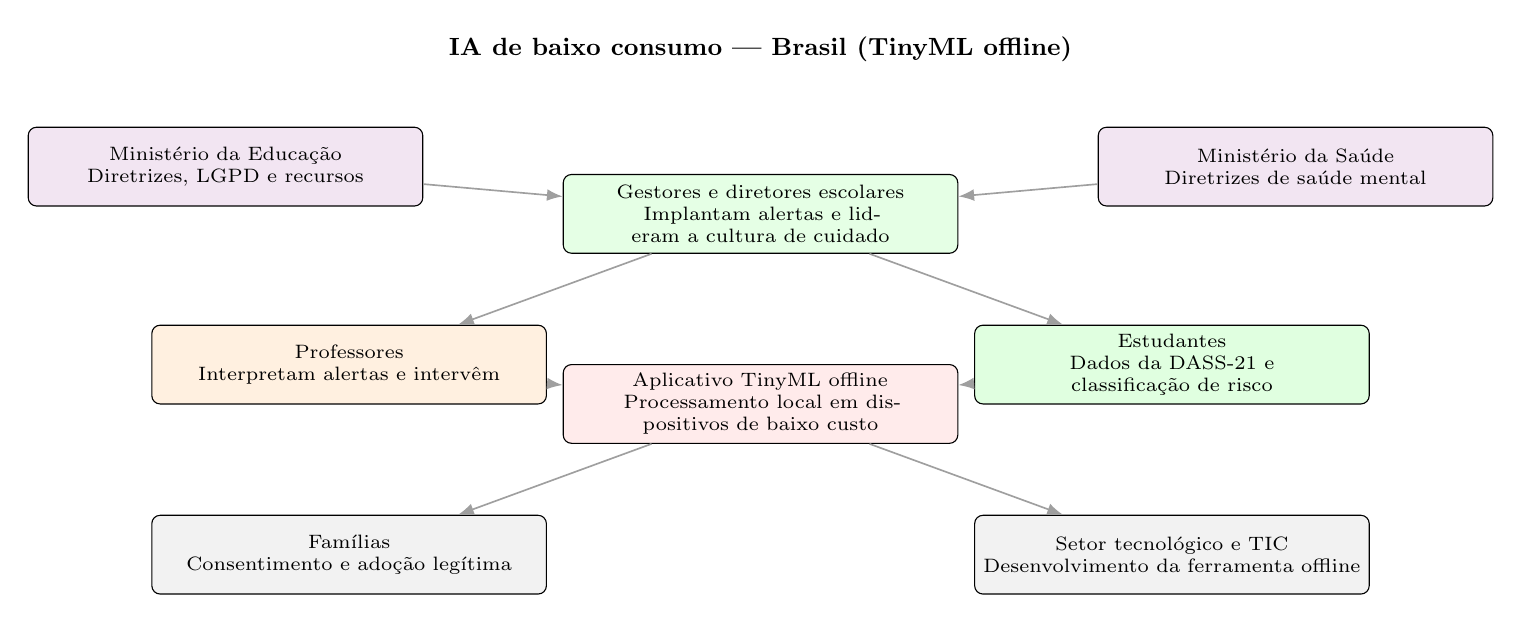
\begin{tikzpicture}[
    node distance=7mm and 10mm,
    every node/.style={font=\scriptsize,align=center},
    caixa/.style={draw,rounded corners=3pt,minimum height=10mm,
      text width=48mm,inner sep=3pt},
    fluxo/.style={-{Latex[length=2mm]},gray!75,semithick}
  ]
    \node[font=\small\bfseries] (titulo)
      {IA de baixo consumo --- Brasil (TinyML offline)};
    \node[caixa,fill=violet!10,below left=7mm and 2mm of titulo] (educacao)
      {Ministério da Educação\\Diretrizes, LGPD e recursos};
    \node[caixa,fill=violet!10,below right=7mm and 2mm of titulo] (saude)
      {Ministério da Saúde\\Diretrizes de saúde mental};
    \node[caixa,fill=green!10,below=13mm of titulo] (gestores)
      {Gestores e diretores escolares\\Implantam alertas e lideram a cultura de cuidado};
    \node[caixa,fill=orange!12,below left=9mm and 2mm of gestores] (professores)
      {Professores\\Interpretam alertas e intervêm};
    \node[caixa,fill=green!12,below right=9mm and 2mm of gestores] (estudantes)
      {Estudantes\\Dados da DASS-21 e classificação de risco};
    \node[caixa,fill=red!8,below=14mm of gestores] (aplicativo)
      {Aplicativo TinyML offline\\Processamento local em dispositivos de baixo custo};
    \node[caixa,fill=gray!10,below left=9mm and 2mm of aplicativo] (familias)
      {Famílias\\Consentimento e adoção legítima};
    \node[caixa,fill=gray!10,below right=9mm and 2mm of aplicativo] (tecnologia)
      {Setor tecnológico e TIC\\Desenvolvimento da ferramenta offline};

    \draw[fluxo] (educacao) -- (gestores);
    \draw[fluxo] (saude) -- (gestores);
    \draw[fluxo] (gestores) -- (professores);
    \draw[fluxo] (gestores) -- (estudantes);
    \draw[fluxo] (professores) -- (aplicativo);
    \draw[fluxo] (estudantes) -- (aplicativo);
    \draw[fluxo] (aplicativo) -- (familias);
    \draw[fluxo] (aplicativo) -- (tecnologia);
  \end{tikzpicture}
  }
  \caption{Atores e relações operacionais da proposta de IA de baixo consumo}
  \label{fig:atores-tinyml}
  \par\smallskip
  \small Fonte: tradução e adaptação de \emph{catedra\_texto.pdf}.
\end{figure}

A Figura \ref{fig:atores-tinyml} mostra a articulação prevista. Educação e saúde
definem diretrizes, recursos e regras; gestores escolares conduzem a implantação
e promovem uma cultura de cuidado; professores interpretam alertas e ajudam a
acionar o fluxo; estudantes fornecem os dados da DASS-21; famílias participam da
legitimação e do cuidado; e parceiros tecnológicos apoiam o desenvolvimento da
solução offline.

\section{Cenário político}

O Brasil já deu um passo legislativo ao instituir a Política Nacional de Atenção
Psicossocial nas Comunidades Escolares por meio da Lei nº 14.819/2024. A norma
reconhece a saúde mental como componente da qualidade educacional e determina a
articulação entre educação, saúde e assistência social \cite{brasil14819}. A
lacuna encontra-se agora na capacidade de implementar o que a política prevê.

A execução, porém, depende de coordenação entre setores e de capacidade local
para acolher os estudantes. A nota técnica aponta um déficit acumulado de
R\$ 117,71 bilhões no chamado Orçamento do Conhecimento desde 2014. Esse dado é
usado no documento para situar as restrições de financiamento que afetam as
redes de ensino. A lei atribui a governança aos Grupos de Trabalho
Intersetoriais do Programa Saúde na Escola e exige a participação da saúde e da
comunidade escolar \cite{brasil14819}. O programa proposto deve partir dessa
estrutura, em vez de criar um fluxo paralelo.

A nota técnica também registra redução de 2,3\% nas matrículas da educação
básica em 2025. Como esse movimento pode decorrer de mudanças demográficas e
administrativas, ele não deve ser interpretado automaticamente como evasão. Os
resultados do programa precisam ser comunicados com a mesma cautela,
distinguindo variação ao longo do tempo, associação e efeito causal.

\section{Atores envolvidos}

Os ministérios e as secretarias de Educação e Saúde ocupam posição central:
definem diretrizes, distribuem recursos e estabelecem regras para que a
ferramenta cumpra a LGPD e as políticas nacionais de saúde mental escolar. Seu
interesse é elevado, pois o tema possui relevância social e potencial retorno
público. A liderança deve ser compartilhada com a assistência social e com as
instâncias territoriais do Programa Saúde na Escola.

Diretores e professores participam da implantação cotidiana e da interpretação
dos alertas. A adesão desses profissionais dependerá de o sistema ser percebido
como apoio, e não como nova forma de cobrança. Isso exige formação para respostas
emocionais, informacionais e instrumentais, além de reorganização das tarefas.
Se apenas acrescentar trabalho, a tecnologia tende a ser abandonada ou utilizada
de maneira superficial.

Os estudantes são o grupo mais afetado. Seu engajamento depende, sobretudo, da
confiança de que os dados não serão utilizados para rotular, discriminar ou
punir. Pais e responsáveis também influenciam a legitimidade do programa. A
comunicação de privacidade deve explicar, em linguagem simples, o que é coletado,
quem pode acessar e quais providências podem ocorrer.

Parceiros tecnológicos, universidades e organizações da sociedade civil podem
fornecer capacidade para construir e adaptar o sistema às condições locais. A
nota técnica menciona organizações especializadas em ferramentas
\emph{offline-first} para o Sul Global. Essas parcerias devem estar subordinadas
à governança pública, com padrões abertos, portabilidade, transparência e
proibição de exploração comercial dos dados estudantis.

\section{Desafios e lacunas}

A proposta enfrenta problemas de naturezas diferentes. Boa parte das soluções
de IA pressupõe uma infraestrutura que muitas escolas não possuem. Ao mesmo
tempo, o subfinanciamento e a falta de profissionais limitam a resposta ao que a
triagem revela. Há ainda o estigma, que pode levar estudantes a esconder o que
sentem mesmo quando existe um canal de escuta.

Nenhuma dessas lacunas é resolvida apenas com um modelo mais preciso. O desafio
tecnológico pede arquitetura local e manutenção simples; o institucional exige
governança, formação e articulação da rede; o sociocultural requer comunicação,
confidencialidade e participação estudantil. É por esse motivo que as
recomendações técnicas são apresentadas em conjunto com medidas institucionais e
de comunicação.

\section{Comparação das alternativas de política}

A nota técnica compara o aplicativo offline com duas alternativas: contratação
universal de profissionais e plataforma dependente de alta conectividade. A
comparação não pretende afirmar que uma alternativa elimina as demais. A
contratação de psicólogos e assistentes sociais continua necessária; o
aplicativo atua como apoio à organização da demanda.

\begin{longtable}{p{3.0cm}p{3.3cm}p{3.3cm}p{3.3cm}}
\caption{Comparação das alternativas apresentadas no artigo}\label{tab:alternativas-artigo}\\
\toprule
\textbf{Alternativa} & \textbf{Adequação técnica} & \textbf{Apoio político} & \textbf{Viabilidade organizacional} \\
\midrule
\endfirsthead
\toprule
\textbf{Alternativa} & \textbf{Adequação técnica} & \textbf{Apoio político} & \textbf{Viabilidade organizacional} \\
\midrule
\endhead
Aplicativo de classificação \emph{offline-first}
& Alta: a solução de baixo consumo responde à limitação de conectividade.
& Média-alta: há interesse público no bem-estar, mas preocupações com privacidade podem gerar oposição.
& Média: requer parceria especializada em TinyML e gestão da carga de trabalho. \\
\addlinespace
Contratação universal de profissionais
& Alta: oferece apoio humano direto e possui fundamento científico.
& Média: custo recorrente e sustentabilidade orçamentária podem gerar resistência.
& Baixa em áreas remotas: há dificuldade de contratar e reter profissionais qualificados. \\
\addlinespace
Plataforma de alta conectividade
& Alta em ambientes com infraestrutura e dados adequados.
& Média-baixa: requer investimento elevado e pode criar dependência tecnológica.
& Baixa em escolas sem internet estável, especialmente em territórios historicamente excluídos. \\
\bottomrule
\end{longtable}

\section{Recomendações}

O artigo recomenda uma política apoiada em IA de baixo consumo,
\emph{offline-first} e TinyML para o monitoramento do bem-estar em contextos de
baixa conectividade. O processamento local em dispositivos de baixo custo amplia
o alcance potencial da política. Sua implementação é organizada em quatro ações
coordenadas.

\subsection{Implementação prática}

A implementação começaria pelo desenvolvimento do aplicativo móvel e por um
piloto de alcance limitado. O sistema coleta dados de bem-estar por meio da DASS-21/EDAE-A, um
questionário de 21 itens que avalia sintomas recentes de depressão, ansiedade e
estresse. Seu uso é de rastreio e monitoramento, sem função diagnóstica. Modelos
leves processam localmente os dados e geram faixas auxiliares de atenção em um
sistema de alertas agregados e anonimizados. A ação da escola continua sujeita
ao julgamento profissional.

O artigo sugere iniciar com aproximadamente cem escolas das regiões Norte e
Nordeste, em articulação com iniciativas de AIED Unplugged e TinyML. A meta
inicial proposta é redução de 15\% nos escores da escala entre a linha de base e
o momento posterior à intervenção. Essa porcentagem é uma hipótese mensurável,
não um resultado garantido. Os dados do piloto serviriam para validar o
desempenho, corrigir protocolos, reduzir riscos e fundamentar eventual expansão
nacional.

\subsection{Institucionalização das rotinas de resposta}

A resposta humana precisa fazer parte da rotina escolar antes que a tecnologia
seja ampliada. Módulos de formação continuada devem preparar professores e equipes
para compreender alertas e oferecer apoio emocional, informacional e
instrumental. Também é necessário impedir que a ferramenta se torne mais um
item na rotina já sobrecarregada: reorganizar tarefas, retirar obrigações
administrativas sem relação com o cuidado e criar incentivos institucionais
influencia a percepção do sistema como apoio ou vigilância.

\subsection{Monitoramento orientado à equidade e à transparência}

A confiança no programa também depende de regras de dados que possam ser
compreendidas e fiscalizadas. Isso inclui armazenamento local cifrado, acesso individual
restrito a profissionais treinados, relatórios agregados e anonimizados para
gestores e proibição clara do uso punitivo ou discriminatório. Essas medidas não
são detalhes posteriores da implantação: constituem uma condição para a
participação dos estudantes e das famílias.

\subsection{Tradução da pesquisa}

Os resultados da pesquisa ainda precisam ser adaptados à rotina das escolas.
Adaptar a DASS-21 ao uso cotidiano da escola, produzir orientações claras para
profissionais não especialistas e acompanhar indicadores quantitativos e
qualitativos permite que a ferramenta seja aprimorada continuamente. Entre os
indicadores quantitativos estão os escores da escala e a permanência escolar;
entre os qualitativos, a percepção da comunidade sobre confiança, acolhimento e
utilidade.

A IA de baixo consumo não resolve a falta de apoio psicossocial nas escolas.
Ela pode ajudar a organizar a procura por atendimento e a identificar situações
que exigem atenção, sobretudo onde a conexão é instável. O resultado, porém,
depende do que acontece depois do alerta: se não houver acolhimento e
encaminhamento, o sistema apenas registrará uma necessidade que a rede continua
sem condições de atender.


\chapter{Objetivos e desenho da política}

\section{Objetivo geral}

Desenvolver uma política pública educacional e um protocolo técnico-operacional,
apoiados por TinyML e arquitetura \emph{offline-first}, para auxiliar o
monitoramento preventivo do bem-estar de adolescentes em escolas públicas de
baixa conectividade, assegurando proteção de dados, supervisão humana,
confidencialidade, equidade e articulação com a rede de cuidado.

\section{Objetivos específicos}

O trabalho tem como objetivos específicos criar uma rotina periódica de escuta
que seja acessível e não estigmatizante, delimitar o uso da EDAE-A/DASS-21 ao
rastreio e desenvolver um aplicativo que funcione sem conexão permanente. O
processamento das respostas deverá ocorrer no próprio dispositivo, com envio
apenas do que for necessário. Alertas individuais ficarão disponíveis somente
para profissionais autorizados, enquanto a gestão receberá indicadores
agregados.

Também se pretende preparar professores, gestores e equipes de referência para
interpretar os alertas sem assumir funções clínicas. O fluxo deverá ligar a
escola às famílias, à saúde, à assistência social e ao Sistema de Garantia de
Direitos. Antes de qualquer expansão, o piloto será avaliado quanto ao
desempenho, à segurança, à carga de trabalho, à confiança dos participantes e
às diferenças de acesso e de erro entre grupos.

\chapter{Metodologia e estratégia de implementação}

\section{Abordagem metodológica}

Este é um projeto aplicado, elaborado a partir de análise documental. A nota
técnica V2 é a fonte de partida e foi confrontada com legislação,
estatísticas oficiais e literatura sobre DASS-21, saúde mental de adolescentes,
AIED Unplugged e ética da inteligência artificial. A proposta prevê um
diagnóstico local, a elaboração conjunta do protótipo, o piloto e sua avaliação.
A ampliação só ocorrerá depois das correções indicadas por essa avaliação.

A metodologia foi organizada em quatro frentes. A primeira cuida do
desenvolvimento e do teste do
aplicativo. As demais tratam da organização da resposta humana, do acompanhamento
da equidade e dos dados e da adaptação da pesquisa à rotina escolar.

\section{Ação 1 -- Implementação prática}

O aplicativo móvel deve funcionar em dispositivo compartilhado da escola. Após
uma explicação apropriada à idade, o estudante responde aos 21 itens da escala e
pode solicitar conversa diretamente. A pontuação e a inferência são realizadas
no aparelho. O TinyML gera uma faixa auxiliar de atenção, inicialmente definida
como baixa, moderada ou elevada. Essa terminologia poderá ser ajustada para
evitar aparência diagnóstica.

Propõe-se um piloto em aproximadamente cem escolas das regiões Norte e Nordeste,
contemplando áreas urbanas, rurais, indígenas e remotas quando houver pactuação e
adaptação cultural adequadas. O número é uma referência de desenho da nota
técnica, não uma autorização automática para coleta. A implantação ocorrerá em
ondas para que erros possam ser corrigidos antes da ampliação.

O piloto terá três modos. No primeiro, testa-se apenas o instrumento, a linguagem
e o fluxo humano. No segundo, o modelo opera silenciosamente: suas saídas não
alteram a fila, mas são comparadas à avaliação humana. No terceiro, após análise
de segurança e equidade, as faixas podem apoiar a priorização. Nenhum estudante
deixa de receber acolhimento por ter escore baixo.

\section{Ação 2 -- Institucionalização da resposta humana}

A nota técnica recomenda organizar a resposta antes de ampliar o uso da
tecnologia. A formação continuada tratará da saúde mental na adolescência e dos
limites da triagem. As atividades incluirão exercícios de escuta,
encaminhamento e gestão de crises, além da discussão de estigma, proteção de
dados e acessibilidade. Casos simulados serão usados para observar como as
equipes aplicam esse conhecimento.

Professores não atuarão como terapeutas. Sua função é acolher, comunicar à equipe
responsável e preservar o estudante. A gestão deverá reorganizar tarefas e
reduzir carga administrativa incompatível com o novo fluxo. O tempo adicional de
trabalho será indicador do piloto. A ferramenta deverá ser suspensa ou sua
frequência reduzida se produzir sobrecarga persistente.

\section{Ação 3 -- Equidade e transparência dos dados}

As respostas identificáveis serão cifradas e mantidas localmente pelo menor
tempo necessário. O acesso individual ficará restrito a profissional treinado e
designado. Diretores e secretarias receberão somente relatórios agregados e
anonimizados, como o número de estudantes que demandaram escuta em determinada
unidade, respeitados limiares mínimos de agregação.

O sistema terá controle de acesso por função, autenticação individual, bloqueio
de sessão, logs, atualização assinada e plano de incidentes. Mudanças no modelo e
nos pontos de corte serão registradas. Estudantes e responsáveis poderão pedir
informação, correção e revisão humana. Será proibido usar os dados para punição,
nota, seleção de turma, policiamento, publicidade ou treinamento comercial.

\section{Ação 4 -- Tradução da pesquisa}

A tradução da pesquisa compreende transformar evidências em orientações
compreensíveis, rotinas sustentáveis e instrumentos públicos. A EDAE-A deverá
ser acompanhada por manual breve para operadores, material de linguagem simples
para estudantes e responsáveis e protocolo de referência e contrarreferência.

O acompanhamento reunirá escores da escala, frequência, permanência, tempo de
resposta e medidas de experiência. Entrevistas e grupos focais avaliarão
confiança, compreensão, estigma, utilidade e efeitos não previstos. A meta de
redução de 15\% nos escores médios entre linha de base e pós-intervenção,
sugerida na nota técnica, será tratada como \textbf{hipótese e parâmetro de
planejamento}. Ela não constitui promessa de eficácia e somente poderá ser
interpretada com controle de perdas, composição da amostra, regressão à média e
outras mudanças contextuais.

\section{Arquitetura do produto}

O estudante terá acesso à escala, a um pedido direto de ajuda e, quando
necessário, a uma versão em papel. A pontuação e o modelo TinyML funcionarão no
dispositivo, sem depender da nuvem. As prioridades individuais aparecerão em
uma fila acessível apenas à equipe autorizada. Nessa fila serão registrados o
responsável pelo atendimento, a providência adotada, o prazo e a situação do
caso, sem incluir narrativa clínica que não seja necessária.

Para os gestores, o sistema produzirá um painel com dados anonimizados e um
limiar mínimo de agregação. A sincronização ocorrerá mais tarde, quando houver
conexão, e transmitirá somente os dados previstos. Versões do sistema, acessos,
incidentes, alterações e pedidos de revisão ficarão registrados para auditoria.

\section{Fluxo de cuidado}

\begin{longtable}{p{2.8cm}p{4cm}p{5.5cm}}
\caption{Níveis operacionais do fluxo de cuidado}\label{tab:fluxo}\\
\toprule
\textbf{Nível} & \textbf{Interpretação} & \textbf{Resposta} \\
\midrule
\endfirsthead
\toprule
\textbf{Nível} & \textbf{Interpretação} & \textbf{Resposta} \\
\midrule
\endhead
Acompanhamento & Sem prioridade computacional, preservado o direito de pedir ajuda. & Ações universais de promoção do bem-estar e nova oportunidade de escuta. \\
\addlinespace
Escuta prioritária & Respostas ou pedido explícito recomendam conversa em prazo pactuado. & Revisão humana, acolhimento, registro mínimo e decisão profissional sobre acompanhamento. \\
\addlinespace
Proteção imediata & Situação grave identificada por qualquer canal. & Acionamento imediato do protocolo humano e da rede competente; nunca aguardar o algoritmo. \\
\bottomrule
\end{longtable}

\section{Indicadores e estratégia de avaliação}

\begin{longtable}{p{2.5cm}p{5cm}p{5cm}}
\caption{Indicadores do piloto}\label{tab:indicadores}\\
\toprule
\textbf{Dimensão} & \textbf{Indicador} & \textbf{Interpretação} \\
\midrule
\endfirsthead
\toprule
\textbf{Dimensão} & \textbf{Indicador} & \textbf{Interpretação} \\
\midrule
\endhead
Alcance & Percentual de estudantes que tiveram oportunidade acessível de participar. & Verifica inclusão, sem transformar adesão em obrigação. \\
Resposta & Tempo mediano entre pedido/sinalização e primeira escuta. & Mede capacidade real da rede. \\
Continuidade & Encaminhamentos com retorno no prazo. & Avalia articulação, sem coletar conteúdo clínico. \\
Bem-estar & Mudança nos escores das subescalas e no total. & Resultado exploratório; não equivale a diagnóstico ou efeito causal isolado. \\
Educação & Frequência, permanência e vínculo escolar. & Análise agregada e longitudinal, com controle de confundidores quando possível. \\
Modelo & Sensibilidade, especificidade, calibração e erros. & Avaliação por contexto e grupo; nenhuma métrica isolada decide expansão. \\
Equidade & Diferenças de acesso, resposta e erro entre grupos. & Disparidades graves determinam suspensão e redesenho. \\
Proteção & Incidentes, acessos indevidos e tempo de resposta. & Avalia segurança e responsabilização. \\
Experiência & Confiança, compreensão, estigma e utilidade percebida. & Inclui estudantes, famílias e profissionais. \\
Trabalho & Tempo adicional e percepção de sobrecarga. & Orienta ajuste de frequência, equipe e escopo. \\
\bottomrule
\end{longtable}

\chapter{Descrição do artefato}

\section{Natureza e finalidade}

O artefato é um pacote técnico-educacional replicável, formado pelo Protocolo
Integrado de Escuta, Triagem e Encaminhamento e pelo protótipo funcional do
aplicativo. Sua finalidade é transformar as recomendações da nota técnica em
procedimentos auditáveis para uma rede pública. O produto une tecnologia,
formação, governança, fluxo de cuidado e avaliação.

\section{Componentes}

O material de implantação compreenderá um caderno de governança, com a divisão
de responsabilidades, e um mapa dos serviços de saúde, assistência e proteção
disponíveis no território. A versão da EDAE-A/DASS-21 e suas instruções só serão
incluídas após autorização técnica. O aplicativo terá processamento local,
acesso individual restrito e um painel gerencial agregado.

O conjunto será completado pelo protocolo de acolhimento, referência e
contrarreferência, pelo material de formação das equipes, pelo relatório de
impacto à proteção de dados e pelo plano de resposta a incidentes. O plano de
avaliação definirá o conteúdo do relatório público do piloto.

\section{Matriz de alternativas}

A nota técnica compara três alternativas segundo correção técnica, apoio
político e viabilidade organizacional. A matriz abaixo preserva essa lógica e
explicita que o aplicativo não substitui a contratação de profissionais.

\begin{longtable}{p{3.2cm}p{3.4cm}p{3.4cm}p{3.4cm}}
\caption{Comparação de alternativas de política}\label{tab:alternativas}\\
\toprule
\textbf{Alternativa} & \textbf{Adequação técnica} & \textbf{Apoio político} & \textbf{Viabilidade organizacional} \\
\midrule
\endfirsthead
\toprule
\textbf{Alternativa} & \textbf{Adequação técnica} & \textbf{Apoio político} & \textbf{Viabilidade organizacional} \\
\midrule
\endhead
Aplicativo \emph{offline-first} & Alta para superar conectividade e estruturar triagem; depende de validação local. & Média-alta: bem-estar tem interesse público, mas privacidade pode gerar oposição. & Média: requer parceria TinyML, governança e gestão de carga. \\
\addlinespace
Contratação universal de profissionais & Alta para cuidado humano direto. & Média: custos recorrentes e sustentabilidade orçamentária são obstáculos. & Baixa a média em áreas remotas pela dificuldade de provimento; continua sendo objetivo complementar. \\
\addlinespace
Plataforma de alta conectividade & Potencial técnico em ambientes conectados. & Média-baixa pelos custos de infraestrutura e dependência. & Baixa em territórios sem conexão adequada. \\
\bottomrule
\end{longtable}

\section{Critérios de aceite}

O piloto somente poderá começar quando a rede tiver pactuado o fluxo e
demonstrado capacidade para atender o número previsto de participantes. Até lá,
os operadores deverão estar formados, o Relatório de Impacto à Proteção de Dados
concluído e a alternativa não digital disponível. A interface precisa ser
testada com adolescentes, e eventuais vulnerabilidades críticas precisam ser
corrigidas. A expansão dependerá dos resultados de utilidade, desempenho,
equidade, proteção e carga de trabalho, além da aprovação do comitê com
participação social.

\chapter{Aspectos éticos, legais e sociais}

\section{Proteção integral e participação}

O Estatuto da Criança e do Adolescente estabelece proteção integral e prioridade
absoluta \cite{brasil8069}. O programa deverá atuar no melhor interesse do
estudante, oferecer informação apropriada à idade e garantir participação na
cocriação e avaliação. A recusa em responder não poderá gerar sanção, suspeita
ou perda de atendimento. Deve existir canal humano independente do aplicativo.

\section{Proteção de dados}

Dados relacionados à saúde e ao estado emocional podem ser pessoais sensíveis.
A LGPD exige finalidade, adequação, necessidade, segurança, prevenção, não
discriminação e responsabilização, além de proteção especial a crianças e
adolescentes \cite{brasil13709}. O controlador deverá documentar a hipótese
legal de cada operação, sem recorrer ao consentimento como justificativa
genérica para todo o tratamento.

O Relatório de Impacto à Proteção de Dados mapeará finalidade, origem, acesso,
compartilhamento, retenção e eliminação. Identificadores ficarão separados dos
dados analíticos. A sincronização privilegiará estatísticas agregadas. O uso
individual será restrito à continuidade do cuidado, e a gestão geral não terá
acesso a nomes.

\section{Ética e justiça algorítmica}

A Recomendação da UNESCO sobre Ética da Inteligência Artificial enfatiza
proporcionalidade, prevenção de danos, privacidade, transparência, auditabilidade,
equidade e supervisão humana \cite{unesco2022}. Esses princípios serão
traduzidos em documentação do modelo, testes por contexto, registro de versões,
explicação das saídas e possibilidade de contestação.

Falsos negativos podem atrasar apoio; falsos positivos podem causar estigma e
sobrecarga. O limiar deve considerar ambos os danos e a capacidade de resposta.
Se o desempenho for insuficiente ou houver disparidade persistente, o componente
de IA será suspenso, mantendo-se o canal humano.

\section{Riscos e mitigação}

\begin{longtable}{p{3.1cm}p{4.4cm}p{5.4cm}}
\caption{Matriz de riscos}\label{tab:riscos}\\
\toprule
\textbf{Risco} & \textbf{Dano possível} & \textbf{Mitigação e resposta} \\
\midrule
\endfirsthead
\toprule
\textbf{Risco} & \textbf{Dano possível} & \textbf{Mitigação e resposta} \\
\midrule
\endhead
Vazamento & Exposição, discriminação e perda de confiança. & Minimização, criptografia, controle de acesso, logs, resposta a incidentes e apoio aos afetados. \\
Falso negativo & Necessidade não reconhecida. & Pedido direto de ajuda, múltiplos canais, reavaliação e vedação de negar acolhimento por escore. \\
Falso positivo & Estigma, ansiedade e sobrecarga. & Saída não clínica, revisão humana, correção e acompanhamento de consequências. \\
Viés & Tratamento desigual. & Validação local, auditoria desagregada, participação diversa e suspensão diante de disparidades graves. \\
Uso punitivo & Violação de direitos. & Proibição normativa, segregação de acesso, auditoria, apuração e reparação. \\
Medicalização & Rotulação de experiências escolares. & Linguagem de bem-estar, análise de contexto e formação sobre limites. \\
Rede insuficiente & Identificação sem resposta. & Mapeamento prévio, piloto limitado, pactuação e interrupção se necessário. \\
Sobrecarga & Atraso e desgaste de trabalhadores. & Dimensionamento, reorganização de tarefas e indicador de carga. \\
Exclusão & Participação desigual. & Acessibilidade, alternativa em papel, suporte e adaptação cultural. \\
Dependência de fornecedor & Custos e descontinuidade. & Código auditável, padrões abertos, portabilidade e plano de saída. \\
\bottomrule
\end{longtable}

\section{Pesquisa com seres humanos}

Se o piloto tiver objetivo de produzir conhecimento generalizável e caracterizar
pesquisa com seres humanos, o protocolo deverá ser submetido ao sistema de ética
em pesquisa aplicável antes do recrutamento. Consentimento do responsável e
assentimento do adolescente serão utilizados quando exigidos, sem confundir
esses documentos com a base jurídica de todas as operações administrativas da
política.

\chapter{Público-alvo e atores}

O público direto é composto por adolescentes dos anos finais do ensino
fundamental e do ensino médio de escolas públicas, especialmente em áreas de
baixa conectividade e oferta limitada de apoio psicossocial. Atores envolvidos
incluem professores, gestores, psicólogos, assistentes sociais, profissionais da
atenção primária e RAPS, famílias, secretarias, conselhos escolares, encarregados
de dados, universidades, organizações da sociedade civil e parceiros técnicos.

\begin{longtable}{p{3.3cm}p{5cm}p{4.5cm}}
\caption{Atores, interesses e responsabilidades}\label{tab:atores}\\
\toprule
\textbf{Ator} & \textbf{Interesse/risco} & \textbf{Responsabilidade} \\
\midrule
\endfirsthead
\toprule
\textbf{Ator} & \textbf{Interesse/risco} & \textbf{Responsabilidade} \\
\midrule
\endhead
Estudantes & Acesso a apoio; risco de estigma e exposição. & Participar do desenho, decidir sobre a escuta e contestar registros. \\
Famílias & Proteção e confiança; preocupação com privacidade. & Participar da comunicação e do cuidado conforme o melhor interesse. \\
Professores & Apoio para agir; risco de sobrecarga. & Acolher, observar e acionar o fluxo, sem atribuição clínica. \\
Equipe especializada & Continuidade do cuidado e qualidade técnica. & Revisar alertas, acolher e encaminhar. \\
Gestão escolar & Clima e permanência; risco de uso indevido. & Organizar rotina, recursos e proteção local. \\
Secretarias & Implementação da política e resultados públicos. & Financiar, regulamentar, articular setores e prestar contas. \\
Parceiros técnicos & Desenvolvimento e manutenção. & Cumprir requisitos, documentar e evitar dependência. \\
Universidades & Avaliação rigorosa e formação. & Validar, auditar e comunicar limites. \\
\bottomrule
\end{longtable}

\chapter{Cronograma e responsabilidades}

\begin{longtable}{p{1.2cm}p{5.6cm}p{2.4cm}p{4cm}}
\caption{Cronograma proposto}\label{tab:cronograma}\\
\toprule
\textbf{Etapa} & \textbf{Atividades} & \textbf{Período} & \textbf{Responsáveis} \\
\midrule
\endfirsthead
\toprule
\textbf{Etapa} & \textbf{Atividades} & \textbf{Período} & \textbf{Responsáveis} \\
\midrule
\endhead
1 & Consolidação do TCC e especificação do artefato. & Set.--dez./2026 & Equipe do projeto. \\
2 & Comitê, mapa da rede e diagnóstico de infraestrutura. & Meses 1--2 & Secretarias e escolas. \\
3 & Protocolo, instrumento, RIPD e plano de incidentes. & Meses 2--3 & Equipe multiprofissional, jurídico e encarregado. \\
4 & Cocriação, protótipo e testes de acessibilidade e segurança. & Meses 3--5 & Equipe técnica e usuários. \\
5 & Formação e simulação dos fluxos. & Meses 5--6 & Formadores e rede de proteção. \\
6 & Primeira onda: fluxo sem IA e modelo silencioso. & Meses 6--8 & Escolas e avaliadores. \\
7 & Segunda onda: piloto assistido e expansão até cerca de cem escolas. & Meses 9--12 & Comitê e equipes locais. \\
8 & Avaliação intermediária e correções. & Mês 13 & Avaliadores independentes. \\
9 & Acompanhamento e avaliação pós-intervenção. & Meses 14--18 & Comitê, universidades e redes. \\
10 & Relatório público e decisão sobre expansão. & Mês 18 & Gestão e instâncias participativas. \\
\bottomrule
\end{longtable}

\section{Responsabilidades acadêmicas}

Ivo Calado responde pela organização geral, pela parte de gestão de políticas
públicas e pela revisão do texto. Rafael Durelli concentra-se no diagnóstico
educacional, no tema do bem-estar e no mapeamento dos atores. Diego Dias é
responsável pela arquitetura TinyML/\emph{offline-first} e pelas questões de
segurança, dados e indicadores.

\chapter{Considerações finais}

O projeto procura levar as recomendações da nota técnica V2 para uma situação
concreta de implementação. Para isso, define quem participa, como ocorre o fluxo
de atendimento, quais dados serão usados e em que condições o piloto poderá
avançar. A proposta não é automatizar o cuidado. O aplicativo serviria apenas
para organizar uma etapa inicial de escuta em escolas com poucos recursos.

O uso da EDAE-A/DASS-21 oferece uma base psicométrica melhor que observações
improvisadas, mas não autoriza diagnóstico. Da mesma forma, TinyML e processamento
local diminuem dependência de conectividade e transferência de dados, porém não
eliminam vieses, erros ou riscos de acesso indevido. As salvaguardas humanas,
jurídicas e institucionais continuam indispensáveis.

O piloto em cerca de cem escolas e a meta exploratória de 15\% de redução dos
escores dão concretude ao plano de avaliação. Esses parâmetros deverão ser
revistos conforme capacidade local e análise ética. A política não poderá ser
considerada eficaz apenas porque o aplicativo funciona ou porque a métrica
melhora. É necessário verificar se estudantes confiam no processo, se recebem
resposta, se não há disparidade, se profissionais não são sobrecarregados e se a
rede consegue sustentar o cuidado.

A IA de baixo consumo pode ser útil nesse cenário, mas não constitui uma
solução independente. Seu uso só se justifica se a decisão permanecer com as
pessoas responsáveis pelo cuidado e se educação, saúde e assistência social
conseguirem atuar em conjunto. A abordagem \emph{offline-first} reduz uma
barreira de infraestrutura. Ainda assim, será preciso acompanhar o uso do
sistema para que a tentativa de ampliar o acesso não transforme a
vulnerabilidade dos estudantes em mais vigilância.

\postextual

\bibliography{referencias}

\iffalse % versão original em inglês suprimida; conteúdo traduzido integrado ao corpo

\chapter{Texto integral do artigo \emph{Low-Power Artificial Intelligence for Monitoring Student Well-Being and Burnout Risk in Low-Connectivity Contexts in Brazil}}

\begin{center}
\textbf{Ivo Calado, Rafael Durelli e Diego Dias}
\end{center}

\section{Current scenario}

Brazilian public schools are struggling with rising levels of student anxiety,
chronic stress, and academic exhaustion, phenomena that deteriorate engagement,
academic achievement, and school retention (Zhang \& Liu, 2025; OECD, 2025a).
Two features of the Brazilian system make this especially difficult to address.
First, mental health remains heavily stigmatised: a PISA supplementary analysis
found that roughly 70\% of young people avoid admitting they are stressed (PISA
Focus Report, 2022), which means the students most in need of support are also
the least likely to disclose it. Second, the institutional capacity to notice
and respond is thin, as only 15.7\% of Brazilian public schools have a
psychologist on site (BRAZIL, 2024; G1, 2025). Therefore, identification and
response depend on the informal, unsystematic judgment of already-overloaded
teachers.

Poor connectivity itself does not cause the problem; it is, however, a
compounding factor. With only 63.7\% of schools in Brazil's North region
connected to the internet (BRAZIL, 2024; TELETIME, 2025), the cloud-based
platforms that dominate the AI in education market are simply not usable in
many of the schools where psychosocial need is greatest (Sarker, 2021; Liu et
al., 2024). The result is a double exclusion: students in low-connectivity
regions face both weaker in-person psychosocial infrastructure and no realistic
path to AI-based support tools designed for high-bandwidth contexts.

\section{Proposed solution}

Addressing this gap requires a tool built for the conditions schools actually
have, not the conditions AI vendors assume. This work proposes an offline-first
mobile application that administers a validated psychosocial screening
instrument, the DASS-21 (Depression, Anxiety and Stress Scale), adapted for
Brazilian adolescents (Cao et al., 2023). Rather than transmitting responses to
a cloud server, the app scores them locally using a lightweight classification
model (TinyML), a form of low-power AI that mirrors the low-connectivity,
minimal-hardware design principles at the core of AIED Unplugged (Uema et al.,
2026). Students complete the questionnaire on a shared school device; the app
classifies each response into a risk band (low, moderate, or severe stress); and
school staff receive an aggregated, anonymised alert, for example ``five
students in this class flagged at moderate-to-severe risk,'' rather than
individually identifying names to anyone outside a trained counsellor's view.

This design choice is deliberate, not incidental. It replaces a slow, informal,
and inconsistent diagnostic process, that currently depends on an overstretched
staff noticing distress on their own, with a fast, structured screening step.
This frees staff time for the part of the process that actually requires a
human: interpretation and support. Since evidence on teacher and student
well-being consistently finds that principal and staff support is one of the
strongest predictors of reduced burnout and stress (Martins, 2020; Carlotto,
2002), the tool is designed to strengthen that human layer, not replace it. For
the same reason, aggregation and confidentiality safeguards are a foundational
need. Research on school-based mental health tools warns that even
well-intentioned monitoring can produce a perverse incentive, with students
concealing distress for fear of being labelled if confidentiality is not
technically guaranteed (Ovi et al., 2026).

\section{Political Landscape}

Brazil has already taken a legislative step in this direction: the National
Policy of Psychosocial Attention in School Communities (Law 14.819/2024)
formally recognises mental health as a component of education quality. The gap
is now implementation capacity. Education, health, and social-assistance sectors
remain fragmented, and chronic underfunding (an accumulated R\$117.71 billion
shortfall in the Knowledge Budget since 2014; Knowledge Observatory, 2023), has
left schools without scalable mechanisms to act on the policy's intent. This is
a case of policy failure through insufficient instruments rather than absence
of diagnosis (Lima \& D'Ascenzi, 2013). At the same time, there is a relevant
political opportunity: Brazil recorded a 2.3\% drop in basic education enrollment
in 2025 (BRAZIL, 2024), and interventions that can demonstrably improve that
behaviour, offering measurable outcomes and positive political response, will
likely be a priority for education authorities.

\section{Stakeholders}

The Ministries of Education and Health hold central authority, setting
guidelines, allocating resources, and establishing regulatory frameworks that
ensure the tool's compliance with Brazil's General Data Protection Law (BRASIL,
2018) and national school mental-health guidance (BRAZIL, 2023); their interest
is high given the political return described above. School principals and
teachers are responsible for day-to-day implementation and interpreting alerts,
but their willingness to adopt the tool depends on it being perceived as
support rather than added workload, which points directly to the need for
training in emotional and instrumental response.

Students are the group most affected, and their engagement hinges on trust,
particularly confidence that data will not be used to label or stigmatise them.
Parents and guardians shape the tool's legitimacy through consent and either
reinforce or resist adoption depending on how privacy is communicated. Finally,
technology partners and civil-society organisations, including groups such as
Nyansa Pol Labs, which specialise in offline-first educational tools for the
Global South (Plancher et al., 2024), provide the technical capacity to build
and adapt the system to local conditions.

\begin{figure}[htbp]
  \centering
  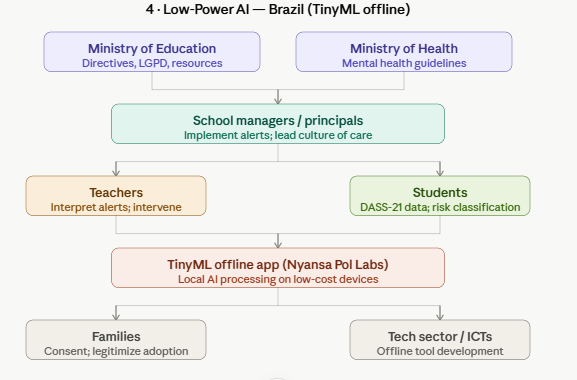
\includegraphics[width=\textwidth]{figuras/comparacao_alternativas_original.png}
  \caption{Stakeholders and operational relationships in the low-power AI proposal}
  \label{fig:stakeholders-original}
  \par\smallskip
  \small Source: extracted from \emph{catedra\_texto.pdf}.
\end{figure}

\section{Challenges and Gaps}

Three structural gaps intersect here. Technologically, most existing AI
solutions were not designed for low-infrastructure environments (Ovi et al.,
2026). Institutionally, chronic underfunding and a shortage of specialised
professionals limit schools' capacity to act on what any screening tool reveals
(Carlotto, 2002). Socioculturally, stigma discourages students from disclosing
distress in the first place. None of these gaps is solved by better technology
alone; each requires a corresponding governance and training response, which is
why the recommendations below pair the technical solution with institutional
and communication measures rather than presenting it in isolation.

\section{Recommendations}

We recommend adopting a public policy built around low-power, offline-first AI
(TinyML) as the core mechanism for monitoring student well-being in
low-connectivity contexts. This approach allows data processing to occur
locally, in low-cost devices, amplifying the policy's reach to historically
excluded regions. Table \ref{tab:comparison-original} compares TinyML to both a
high-connectivity alternative and in-person counselor hiring, analysing its
suitability for the Global South.

\begin{longtable}{p{3.0cm}p{3.3cm}p{3.3cm}p{3.3cm}}
\caption{Comparison of policy alternatives in the original article}\label{tab:comparison-original}\\
\toprule
\textbf{Alternative} & \textbf{Technically correct} & \textbf{Politically supportable} & \textbf{Organizationally implementable} \\
\midrule
\endfirsthead
\toprule
\textbf{Alternative} & \textbf{Technically correct} & \textbf{Politically supportable} & \textbf{Organizationally implementable} \\
\midrule
\endhead
Offline-First Classification App
& HIGH: Low-power solution resolves the connectivity challenge.
& MEDIUM-HIGH: High public interest in well-being, but risk of opposition due to privacy concerns.
& MEDIUM: Requires specialized partnership (TinyML) and management of teacher/staff workload. \\
\addlinespace
Universal Counselor Hiring
& HIGH: Direct support solution and scientifically proven.
& MEDIUM: Opposition due to high recurring cost and budgetary sustainability.
& LOW: Difficulty in finding and retaining qualified professionals in low-income rural areas. \\
\addlinespace
High-Connectivity Platform
& HIGH: High diagnostic accuracy with Big Data.
& MEDIUM-LOW: High cost and political resistance to large infrastructure investments.
& LOW: Lack of internet infrastructure in schools makes it unfeasible for the Global South. \\
\bottomrule
\end{longtable}

This could be implemented through four coordinated actions:

\subsection{Practical Implementation}

First, pilot and scale carefully. We argue for the development of an
offline-first mobile application, capable of collecting data about students'
well-being from a validated psychometric instrument (DASS-21) --- a 21 item
questionnaire that assesses levels of depression, anxiety, and stress,
identifying recent emotional state in educational and health research, allowing
screening and monitoring without diagnostic function, adapted and validated for
Brazilian adolescents. The application processes questionnaire data locally
through lightweight machine learning models, classifying students into risk
levels as an aggregated and anonymized alert system, guiding schools' action
without replacing professional judgment.

Implementation should begin with around 100 schools in the Northeast and North
regions, aligned with existing AIED Unplugged and TinyML pilot initiatives, with
a clear, measurable target: a 15\% reduction in DASS-21 scores pre- to
post-intervention (Ovi et al., 2026). Thereon, pilot results can be used to
validate accuracy and refine protocols before expanding nationally, which both
reduces technical risk and builds the political case for scale-up.

\subsection{Institutionalize AI-based pedagogical routines for teachers}

Second, institutionalise the human response, not just the technology.
Continuing-education modules should train teachers and school teams to interpret
alerts and respond with emotional, informational, and instrumental support
(Carlotto, 2002). Equally important is ensuring the tool does not become one
more item on an already-overloaded plate: reorganising tasks, reducing unrelated
administrative burden, and offering institutional incentives will determine
whether staff experience the system as support or surveillance.

\subsection{Building Monitoring with Focus on Equity and Data Transparency}

Third, build trust through data governance, explicitly and visibly. Local,
encrypted storage; individual-level access restricted to trained counsellors;
aggregated, anonymised reporting for managers; and an explicit, communicated
prohibition on using the data for punitive or discriminatory purposes are not
implementation details, they are the precondition for student and family
participation, given the stigma documented above.

\subsection{Research Translation}

Fourth, invest in research translation. Adapting DASS-21 for everyday school
use, producing clear guidance for non-specialist staff, and tracking both
quantitative indicators (DASS-21 scores, dropout rates) and qualitative signals
(school-community perception) will determine if the tool is able to become a
genuine, evolving instrument of care.

Taken together, these measures reframe the central claim of this case study:
although low-power AI is not, by itself, a solution to student well-being in
Brazil, it is a way of making an already understood and legislated problem (the
absence of systematic, trusted, and timely psychosocial support) tractable in
the schools that today have the least capacity to address it.

\fi

\end{document}
